\documentclass[xcolor=table]{beamer}
\usepackage[utf8]{inputenc}
\usepackage[british]{babel}
\usepackage[super]{nth}
%\usetheme{Boadilla}
%\usecolortheme{rose}
%\usecolortheme{crane}
%\usefonttheme{structuresmallcapsserif}
%\setbeamertemplate{navigation symbols}{}

\definecolor{Main}{rgb}{0.74, 0.13, 0.19}
\definecolor{Accent1}{rgb}{0.76,0.36,0.13}
\definecolor{Accent2}{rgb}{0.54,0.1,0.4}

\mode<presentation>{\usetheme{ilm}}
%\usecolortheme{rose}
%\useinnertheme[shadow]{circles}
%\usecolortheme{whale}
%\useoutertheme{infolines}

%\usecolortheme[named=Accent1]{structure}




%\setbeamerfont{page number in head/foot}{size=\large}
%\setbeamercolor{page number in head/foot}{fg=Main}
%% page/total
%%\setbeamertemplate{footline}[frame number]
%% pas de total
%\setbeamertemplate{footline}{%
%    	\hfill%
%	\usebeamercolor[fg]{page number in head/foot}%
%	\usebeamerfont{page number in head/foot}%
%	\insertframenumber\kern1em\vskip2pt%
%}
%
%\setbeamersize{text margin left=1em}
%\setbeamersize{text margin right=1em}

\usepackage[overlay,absolute]{textpos}
\setlength{\TPHorizModule}{10mm}
\setlength{\TPVertModule}{\TPHorizModule}
\textblockorigin{10mm}{10mm} % start everything near the top-left corner
\setlength{\parindent}{0pt}

%font
\usepackage[T1]{fontenc}
\usepackage{times}
%\usepackage[oldstylenums]{kpfonts}

%\include{macros}
\usepackage{ifthen}


%proper math and math symbols
\usepackage{amsmath,mathtools}
\usepackage{amssymb}

\usepackage{datenumber,fp}

\usepackage[separate-uncertainty = true]{siunitx}

\usepackage{tabu}
\usepackage{multirow}
\usepackage{booktabs}

% Allow the usage of graphics (.jpg, .png, etc.) in the document
\usepackage{graphicx}
\usepackage{tikz}
\usetikzlibrary{arrows,shapes,backgrounds, calc, positioning, topaths,chains, intersections, decorations.markings, decorations.text, shapes.geometric, matrix,patterns,mindmap}
%\usetikzlibrary{positioning, patterns,topaths,chains,matrix}

\usepackage{pgfplots}
\usepackage{pgfplotstable}
\pgfplotsset{compat=1.9}
\usepgfplotslibrary{groupplots}
\usepgfplotslibrary{external}
\makeatletter
\newcommand*{\overlaynumber}{\number\beamer@slideinframe}
\tikzset{
  beamer externalizing/.style={%
    execute at end picture={%
      \tikzifexternalizing{%
        \ifbeamer@anotherslide
        \pgfexternalstorecommand{\string\global\string\beamer@anotherslidetrue}%
        \fi
      }{}%
    }%
  },
  external/optimize=false
}
\let\orig@tikzsetnextfilename=\tikzsetnextfilename
\renewcommand\tikzsetnextfilename[1]{\orig@tikzsetnextfilename{#1-\overlaynumber}}
\makeatother

\tikzset{every picture/.style={beamer externalizing}}
\tikzexternalize
\tikzsetexternalprefix{fig_presentation/}
%\tikzset{external/optimize=false}
%\tikzset{external/force remake}


%link or play movies
\usepackage{multimedia}

%chemistry
\usepackage[version=3]{mhchem}
\usepackage{chemfig}
\usepackage{setspace}


%beamer related package

\usepackage{todonotes}
\presetkeys{todonotes}{inline}{}

\tikzset{onslide/.code args={<#1>#2}{%
  \only<#1>{\pgfkeysalso{#2}} %
}}%


%bibliography
\usepackage[style=authoryear-comp, language=british,eprint=false, url=false, doi=false, sortcites=true, sorting=none, isbn=false, firstinits=true,maxcitenames=6]{biblatex}
%minimal citations
\AtEveryCitekey{%
	\clearfield{title}
	\clearfield{pages}
	\clearfield{volume}
	\clearfield{number}
	\clearfield{month}}
\newcommand{\myfullcite}[1]{{\scriptsize\fullcite{#1}}}
\renewbibmacro{in:}{%
  \ifentrytype{article}{}{%
  \printtext{\bibstring{in}\intitlepunct}}}
%\bibliography{biblio}


\newcolumntype{P}[1]{>{\raggedright}p{#1}}

\institute[iLM]{Univ Lyon, Université Claude Bernard Lyon 1, CNRS, Institut Lumière Matière}
\title[processionary gel]{Ion pairing controls rheological properties of ``processionary'' polyelectrolyte hydrogels}
\author[M. Leocmach]{Mathieu Leocmach {\usebeamerfont{normal text}\texttt{\usebeamercolor[fg]{normal text}\footnotesize @LamSonLeoc}}\vspace{-\baselineskip}}
\date{%10 August 2016
}
\titlegraphic{\vspace{-\baselineskip}
	\begin{tabu}{X[c]X[c]X[c]X[c]}
		\multicolumn{2}{c}{\usebeamerfont{institute}\usebeamercolor[fg]{institute}ENS de Lyon, Laboratoire de Chimie}&
		\multicolumn{2}{c}{\usebeamerfont{institute}\usebeamercolor[fg]{institute}ENS de Lyon, Laboratoire de Physique}\\\cmidrule(r){1-2}\cmidrule(l){3-4}
		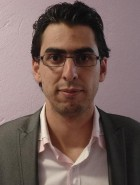
\includegraphics[height=3\baselineskip]{presentation/Hassan}&
		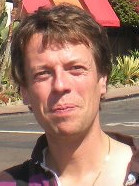
\includegraphics[height=3\baselineskip]{presentation/Cyrille}&
		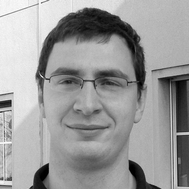
\includegraphics[height=3\baselineskip]{presentation/Nicolas_Taberlet}&
		\includegraphics[height=3\baselineskip]{../Yaourt/Seb}\\
		Hassan & Cyrille & Nicolas & S\'{e}bastien\\
		Srour & Monnereau & Taberlet & Manneville\\\cmidrule(r){1-2}
		\multicolumn{2}{c}{Martien Duvall Deffo Ayagou}&\\
		\multicolumn{2}{c}{Thi Thanh-Tam Nguyen}&\raisebox{-0.1em}[0pt][0pt]{
\includegraphics[height=2\baselineskip]{presentation/invest-avenir.jpg}}&\raisebox{-0.1em}[0pt][0pt]{\includegraphics[height=2\baselineskip,clip=true, trim=6mm 14mm 6mm 0]{../Yaourt/NEW-Logo-ERC-OUTLINE}}\\
	\end{tabu}
	
\bigskip
Martien Duvall Deffo Ayagou, Thi Thanh-Tam Nguyen%, Chantal Andraud
	
	%\vfill
	%\includegraphics[height=2\baselineskip]{logo_ens-lyon}\quad
	%\includegraphics[height=2\baselineskip]{logo_ums_grand}\quad
	%\includegraphics[height=2\baselineskip]{../../Yaourt/CNRSfilaire-Q}\quad
	%\includegraphics[height=2\baselineskip]{CRPP}\quad
	%\includegraphics[height=2\baselineskip,clip=true, trim=6mm 14mm 6mm 0]{NEW-Logo-ERC-OUTLINE}
	}


\newlength{\mylength}

%\includeonly{creep_beamer}

\begin{document}
\tikzset{every mark/.append style={scale=0.8}}
\pgfplotsset{every axis/.append style={footnotesize}}

\pgfplotscreateplotcyclelist{earthy}{%
{red!40!black,mark=o},
{red!60!black,mark=triangle, every mark/.append style={rotate=180}},
{red!80!black,mark=square},
{red,mark=triangle},
{red!80!yellow, mark=diamond},
red!60!yellow,
red!40!yellow,
}

\AtBeginSection[]{
	\addtocounter{framenumber}{-1}
	\begin{frame}[plain]
		\tableofcontents[currentsection, hideothersubsections]
	\end{frame}
}

\begin{frame}{\pgfuseimage{cnrs-logo}\hspace*{0.3cm}\pgfuseimage{ucbl-logo}\pgfuseimage{univlyon-logo}}%[plain]
	\titlepage
\end{frame}

\setcounter{framenumber}{0}

\begin{frame}{Fine chemistry}
	\vspace{\baselineskip}
	\tikzsetnextfilename{polymerisation}%
	\let\mrad\relax%
	\newlength\mrad%
	\setlength{\mrad}{1ex}%
	% The face style, can be changed
	\tikzset{face/.style={
		shape=circle,minimum size=2\mrad,shading=radial,outer sep=0pt,
	    inner color=white!50!yellow,outer color= yellow!70!orange
		}}%
	\begin{tikzpicture}
		\foreach \i [evaluate=\i as \dist using \i*0.45] in {0,1,2}{
			\begin{scope}[xshift=\dist\textwidth]
			%face
			\begin{scope}[face/.style={
		shape=circle,minimum size=2\mrad,shading=radial,outer sep=0pt,
	    inner color=white!50!yellow,outer color= yellow!70!orange
		}]
\node[face,inner color=white!50!ilmcolor,outer color= ilmcolor!90!black] (emoticon) {};
			%% The eyes are fixed.
			\draw[fill=white] 
				(-0.5\mrad,0ex) ..controls (-0.25\mrad,0.1\mrad)and(0.25\mrad,0.1\mrad)..
		        (0.5\mrad,0.0pt) ..controls (0.75\mrad,0.75\mrad)and(0.1\mrad,0.85\mrad)..
		        (0pt,0.2\mrad) ..controls (-0.1\mrad,0.85\mrad)and(-0.75\mrad,0.75\mrad)..
		        (-0.5\mrad,0pt)--cycle;
			%% standard pupils
			\node[fill, ellipse,inner xsep=0.075\mrad, inner ysep=0.0375\mrad, rotate=80] at (0.25\mrad,0.25\mrad) {};
			\node[fill, ellipse,inner xsep=0.075\mrad, inner ysep=0.0375\mrad, rotate=100] at (-0.25\mrad,0.25\mrad) {};
			%% mouth
			\draw[thick,line cap=round] (-0.5\mrad,-0.5\mrad)
			     ..controls (-0.25\mrad,-0.75\mrad)and(0.25\mrad,-0.75\mrad)..(0.5\mrad,-0.5\mrad);
\end{scope}
;
			%% horns
			\draw[every node/.style={shape=circle,inner sep=0.2\mrad,shading=radial,inner color=white!50!ilmcolor,outer color= ilmcolor!90!black}] (emoticon.70) -- ++(70:0.4\mrad) node{} (emoticon.110) -- ++(110:0.4\mrad) node{};
			%\draw ( emoticon.80)..controls ( 0.3\mrad,1.2\mrad)..(0.5\mrad,1.25\mrad)
			      %..controls ( 0.4\mrad,1.15\mrad)..(emoticon.70);
			%\draw (emoticon.100)..controls (-0.3\mrad,1.2\mrad)..(-0.5\mrad,1.25\mrad)
			      %..controls (-0.4\mrad,1.15\mrad)..(emoticon.110);
			%body segments
			\ifthenelse{\i=0}{}{
			\foreach \x in {0,2,...,10}{
				\node[face,inner color=white!50!gray,outer color= gray!90!black, left=\x\mrad of emoticon] (monomer){};
				%legs
				\ifthenelse{\i=1}{}{
					\draw[line width=0.25\mrad, ilmorange] (monomer.south) ++(0,0.5\mrad) to[bend left] +(0,-1\mrad);}
			};}
			\ifthenelse{\i=1}{
				\draw[|-|] ($(monomer.west)+(0,-1.5\mrad)$) -- ($(emoticon.west)+(0,-1.5\mrad)$) node[midway,below, font=\scriptsize] {$N_0$};
			}{}
			\end{scope}
			};
			%arrows
			\draw[-stealth, thick] ++(3\mrad,0) -- +(6\mrad,0) node[midway, above=0.2\mrad, face,inner color=white!50!gray,outer color= gray!90!black]{} node[midway, below, font=\scriptsize]{ATRP};
			\draw[-stealth, thick] ++(0.45\textwidth,0) ++(3\mrad,0) -- +(6\mrad,0) coordinate[midway, above=0.2\mrad] (leg) node[midway, below, font=\scriptsize,text width=10\mrad,align=center]{post-functionalization};
			\draw[line width=0.25\mrad, ilmorange] (leg) to[bend right] +(0,1\mrad);
		\end{tikzpicture}

	\bigskip
	\tikzsetnextfilename{polymerisation_PImBr}%
	\definesubmol{head}{(-[::-105,,,,ilmcolor])(-[::-15,,,,ilmcolor])-[::60,,,,ilmcolor](=[::60,,,,ilmcolor]\textcolor{ilmcolor}{O})-[::-60,,,,ilmcolor]\textcolor{ilmcolor}{O}-[::-60,,,,ilmcolor]-[::60,,,,ilmcolor]-[::60,,,,ilmcolor]}
\definesubmol{mono}{-[::-60,,,,gray](=[,,,,gray]\textcolor{gray}{O})-[::-60,,,,gray]\textcolor{gray}{O}-[::60,,,,gray]-[,,,,gray]-[::-60,,,,gray]}
\tikzsetnextfilename{polymerisation_PImBr}
\begin{tikzpicture}[every node/.style={font=\tiny\setatomsep{1.5em}}]
	\node (init) {\chemfig{Br-[:-30]!{head}\textcolor{ilmcolor}{P}|\textcolor{ilmcolor}{O_3}Et_2}};
	
	\node[below left=5\baselineskip and 0 of init.east] (POH) {%
	\chemfig{[:-30]-[@{left,0.25}](%
		!{mono}OH%
		)-[::60,,,,gray]-[@{right,0.25}]!{head}\textcolor{ilmcolor}{P}|\textcolor{ilmcolor}{O_3}Et_2}%
	};
	\node[below right=-0.6em and -0.25em of POH.base west] {$\prescript{}{N_0}{\left[\vrule height 1em depth 0.25em width 0pt\hspace{1.75em}\right]}$};
	\node[below right=-0.6em and -0.25em of POH.base west] {};
	
	\node[right=0.1\textwidth of init.base east, anchor=base west] (PBr) {%
	\chemfig{[:-30]-[@{left,0.25}](%
		!{mono}Br%
		)-[::60,,,,gray]-[@{right,0.25}]!{head}\textcolor{ilmcolor}{P}|\textcolor{ilmcolor}{O_3^{2-}}}%
	};
	\node[below right=-0.6em and -0.25em of PBr.base west] {$\prescript{}{N_0}{\left[\vrule height 1em depth 0.25em width 0pt\hspace{1.75em}\right]}$};
	
	\node[right=\textwidth of init.base-|POH.west, anchor=base east] (PNuBr) {%
	\chemfig{[:-30]-[@{left,0.25}](%
		!{mono}\textcolor{ilmorange}{N}|^{\color{ilmorange}+}*5(=[,,,,thick, ilmorange]-[,,,,thick, ilmorange]\textcolor{ilmorange}{N}(-[,,,,thick, ilmorange])-[,,,,thick, ilmorange]=[,,,,thick, ilmorange]-[,,,,thick, ilmorange])(-[0,2,,,draw=none]Br^{-})
		)-[::60,,,,gray]-[@{right,0.25}]!{head}\textcolor{ilmcolor}{P}|\textcolor{ilmcolor}{O_3^{2-}}}%
	};
	\node[below right=-0.6em and -0.25em of PNuBr.base west] {$\prescript{}{N_0}{\left[\vrule height 1em depth 0.25em width 0pt\hspace{1.75em}\right]}$};
	
	\draw[-stealth, thick] (init.south-|POH.north) -- (POH) node[midway, left=0, -]{\chemfig{[:-30]=[,,,,gray]!{mono}OH}} node[midway, right=0, text width=0.13\textwidth, align=center]{\ce{CuBr}\linebreak 4-4'-bipyridine\linebreak \SI{85}{\celsius}};
	\draw[-stealth, thick] (POH) -| (PBr) node[pos=0.25, above]{\ce{TMS-Br}} node[pos=0.25, below, sloped, text width=0.2\textwidth, align=center]{\ce{CH2Cl2}\linebreak \SI{85}{\celsius}};
	\draw[-stealth, thick] (PBr) -- (PBr-|PNuBr.west) node[midway, above,align=center,-]{\chemfig[thick, ilmorange]{[2]*5(-N(-)-=N-=)}} node[midway, below, text width=0.2\textwidth, align=center]{THF\linebreak \SI{85}{\celsius}};;
	\node[anchor=south east] at (POH.south east) {\ce{POH}};
	\node[anchor=south east] at (PBr.south east) {\ce{PBr}};
	\node[anchor=south east] at (PNuBr.south east) {\ce{PIm+Br-}};
	\node[anchor=south east, font=\footnotesize] at (POH.south-|PNuBr.east) {$N_0=70$ from NMR};
\end{tikzpicture}
\end{frame}

\begin{frame}{Physical polyelectrolytes hydrogel}
	\tikzsetnextfilename{polyelectrolytes}%
\begin{tikzpicture}
\let\mrad\relax%
\newlength\mrad%
\setlength{\mrad}{0.45em}%
\draw[every node/.style={circle,draw,font=\tiny, inner sep=0,minimum height=0.5em}] (0,0) --(30:\mrad) node[above right,ilmcolor]{-} (0,0)--(-30:\mrad) node[below right,ilmcolor]{-} (0,0)--++(-180:\mrad)\foreach \x [evaluate=\x as \r using 1/(rnd+0.1), evaluate=\x as \rr using 1/(rnd+0.1)] in {1,2,...,35}{--++(150:\mrad)node[above,ilmorange]{+} node[above=\r\mrad]{-}--++(-150:\mrad)node[below=0,ilmorange]{+} node[below=\rr\mrad]{-}};
\end{tikzpicture}%
\begin{columns}
\column{0.5\textwidth}
\structure{Reversible gel}
\begin{itemize}
	\item in deionised, neutral water
	\item yield stress fuild
\end{itemize}
\structure{Solution} if
\begin{itemize}
	\item ionic strength, pH
	\item non ionic head
\end{itemize}
$\Rightarrow$ Head-to-body ionic bonds

\column{0.5\textwidth}
\hfill Herschel-Buckley law\\
\hfill $\sigma =\sigma_c + A \dot{\gamma}^n$
\tikzsetnextfilename{flowcurves}%
\begin{tikzpicture}
    \let\mrad\relax%
	\newlength\mrad%
	\setlength{\mrad}{0.5em}%
% The face style, can be changed
	\tikzset{face/.style={
		shape=circle,minimum size=2\mrad,shading=radial,outer sep=0pt,
	    inner color=white!50!yellow,outer color= yellow!70!orange
		}}%
\let\drawcaterpillar\relax
\newcommand\drawcaterpillar{
			%face
			\node[face,inner color=white!50!ilmcolor,outer color= ilmcolor!90!black] (emoticon) {};
			%% The eyes are fixed.
			\draw[fill=white] 
				(-0.5\mrad,0ex) ..controls (-0.25\mrad,0.1\mrad)and(0.25\mrad,0.1\mrad)..
		        (0.5\mrad,0.0pt) ..controls (0.75\mrad,0.75\mrad)and(0.1\mrad,0.85\mrad)..
		        (0pt,0.2\mrad) ..controls (-0.1\mrad,0.85\mrad)and(-0.75\mrad,0.75\mrad)..
		        (-0.5\mrad,0pt)--cycle;
			%% standard pupils
			\node[fill, ellipse,inner xsep=0.075\mrad, inner ysep=0.0375\mrad, rotate=80] at (0.25\mrad,0.25\mrad) {};
			\node[fill, ellipse,inner xsep=0.075\mrad, inner ysep=0.0375\mrad, rotate=100] at (-0.25\mrad,0.25\mrad) {};
			%% mouth
			\draw[thick,line cap=round] (-0.5\mrad,-0.5\mrad)
			     ..controls (-0.25\mrad,-0.75\mrad)and(0.25\mrad,-0.75\mrad)..(0.5\mrad,-0.5\mrad);
			
%body segments
			\foreach \x in {0,2,...,4}{
				\node[face,inner color=white!50!gray,outer color= gray!90!black, left=\x\mrad of emoticon] (monomer){};
				%legs
				\draw[line width=0.25\mrad, ilmorange] (monomer.south) ++(0,0.5\mrad) to[bend left] +(0,-1\mrad);
			};
}
\begin{loglogaxis}[
	name=ax,
	xlabel=$\dot\gamma\,(\si{\per\second})$,
	ylabel={$\sigma$ (\si{\pascal)}},
	clip marker paths=true,
	]
	\addplot+[mark=o] table[x=shear_rate, y=shear_stress] {data/PO3-P60-Im+-0pc-02-06-14_8pcw_flow curve_down.txt};
	\addplot+[mark=square] table[x=shear_rate, y=shear_stress] {data/PO3-P60-Im+-0pc-02-06-14_22pcw_flow curve_down.txt};
	\addplot+[black] table[x=shear_rate, y=shear_stress,skip coords between index={0}{20}] {data/Et-P60-Im+-0pc-21-05-14_10pcw_flow_curve_down.txt};
	\addplot[domain=2e-2:5e2]{0.47+1.19*x^0.7};
	\addplot[domain=2e-2:5e2]{7.5+15.1*x^0.62};
\end{loglogaxis}

\begin{scope}[shift=(ax.north), yshift=-2\mrad, xshift=-\mrad]
			\drawcaterpillar
			%% horns
			\draw[every node/.style={shape=circle,inner sep=0.2\mrad,shading=radial,inner color=white!50!ilmcolor,outer color= ilmcolor!90!black}] (emoticon.70) -- ++(70:0.4\mrad) node{} (emoticon.110) -- ++(110:0.4\mrad) node{};
\end{scope}
\begin{scope}[shift=(ax.south), yshift=2\mrad, xshift=-\mrad]
			\drawcaterpillar
\end{scope}
\end{tikzpicture}
\end{columns}
\vspace{-\baselineskip}\textit{\scriptsize Srour et al. Macromol. Rapid Comm., 36, 55 (2015)}
\end{frame}

\begin{frame}{Linear rheology}
	\begin{columns}
	\column{0.5\textwidth}
	\tikzsetnextfilename{linear_rheology_PImBr}%
	\begin{tikzpicture}
	\pgfplotscreateplotcyclelist{moduli}{
		black, mark=*\\%
		black, mark=square\\%
	}
	\begin{loglogaxis}[
		ylabel={moduli (\si{\pascal})},
		xlabel={frequency (\si{\hertz})},
		cycle list name=moduli,
		ytickten={0, 1}, yticklabels={1,10},
		]
		\addplot table[x expr={\thisrow{angfrequency}/6.28}, y=G']{ImBr_70_PO3_8pc_ter.freq} node[midway, above left]{$G^\prime$};
		\addplot table[x expr={\thisrow{angfrequency}/6.28}, y=G'']{ImBr_70_PO3_8pc_ter.freq}  node[midway, below right]{$G^{\prime\prime}$};
		\node[anchor=north west, font=\footnotesize] at (rel axis cs:0,1){8\% wt};
	\end{loglogaxis}
\end{tikzpicture}
	\[ G = \frac{c}{N}k_\mathrm{B}T \]
	\begin{description}[$N$]
	\item[$c$] monomer concentration
	\item[$N$] \# monomers between CL
	\end{description}
	\column{0.45\textwidth}
	\pause
	\begin{itemize}
	\item $N \approx 800 N_0$ !
	\item 800 chains between CL
	\end{itemize}
	\begin{flushright}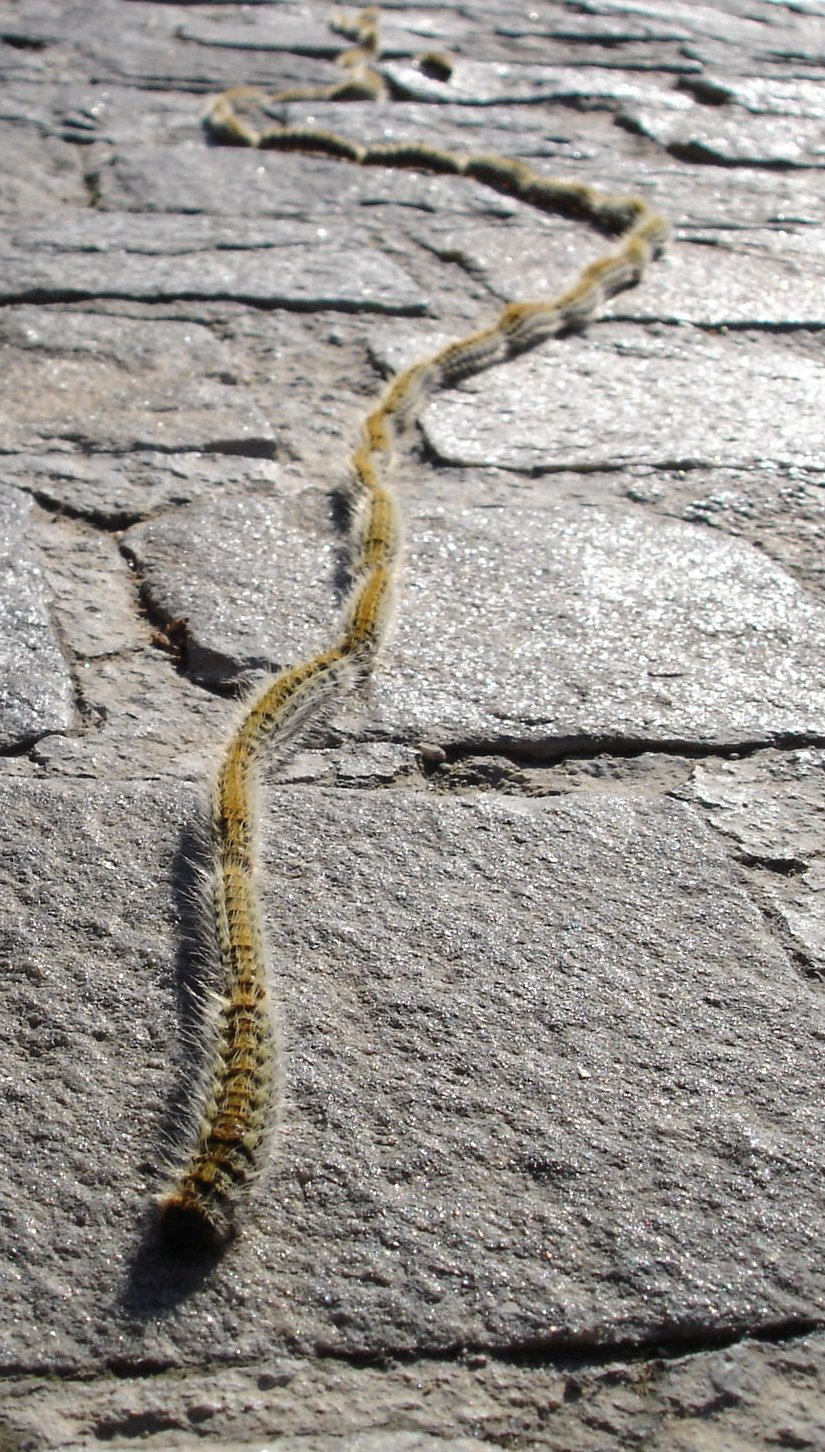
\includegraphics[height=14\baselineskip]{presentation/Thaumetopea_pityocampa_01.jpg}\\
	\vspace{-1.5em}\colorbox{lightgray}{\scriptsize Wikimedia commons}
	\end{flushright}
	\end{columns}
\end{frame}

\end{document}